\documentclass[aspectratio=169, 10pt]{beamer}
\usetheme{Madrid}
\usefonttheme{professionalfonts}

\usepackage[english]{babel}
\usepackage[linguistics]{forest}
\usepackage[utf8]{inputenc}
\usepackage{algorithmic}
\usepackage{amsfonts}
\usepackage{amsmath}
\usepackage{amssymb}
\usepackage{array}
\usepackage{bookmark}
% \usepackage{boondox-cal}
\usepackage{caption}
\usepackage{colortbl}
\usepackage{csquotes}
\usepackage{graphicx}
\usepackage{hyperref}
\usepackage{lipsum}
\usepackage{lmodern}
\usepackage{mathptmx}
\usepackage{mathtools}
\usepackage{multirow}
\usepackage{pgfplots}
\usepackage{svg}
\usepackage{xcolor}

% \pgfplotsset{compat=1.17}
\usetikzlibrary{calc}

\DeclareMathOperator*{\argmax}{argmax}

\hypersetup{
    colorlinks=true,
    linkcolor=blue,
    filecolor=blue,      
    urlcolor=blue,
}

\title{Tutorial 7}
\subtitle{Tutorial on Naive Bayes}
\author{Ben Halstead, Luke Chang}
\institute{The University of Auckland}
\date{May 2021}


\begin{document}

\frame{\titlepage}

% %-------------------------------------------------------------------------------
\begin{frame}
    \frametitle{Topics}

    \tableofcontents
        
\end{frame}

%-------------------------------------------------------------------------------
\section{Multinomial Naive Bayes Classifier}
\begin{frame}[t]
\frametitle{Example 1 - Multinomial Naive Bayes Classifier}
    \begin{example}
        You come to Fiji for a holiday. 10 days later, you realise the weather forecast here isn't very accurate.
        Based on the information you gettered so far and today's weather report, you want to know ``Will it rain this afternoon?''
    \end{example}

    \begin{table}[]
        \small
        \begin{tabular}{l|llll|l}
        \textbf{Day} & \textbf{Outlook} ($O$) & \textbf{Temperature} ($T$) & \textbf{Humidity} ($H$) & \textbf{Wind} ($W$) & \textbf{Rain} ($R$) \\ \hline
        1            & Sunny            & Hot                  & High              & Weak          & True           \\
        2            & Sunny            & Hot                  & High              & Strong        & False            \\
        3            & Overcast         & Hot                  & High              & Weak          & True           \\
        4            & Rain             & Mild                 & High              & Weak          & True           \\
        5            & Rain             & Cool                 & Normal            & Weak          & True           \\
        6            & Rain             & Cool                 & Normal            & Strong        & False            \\
        7            & Overcast         & Cool                 & Normal            & Strong        & False            \\
        8            & Overcast         & Mild                 & High              & Strong        & True           \\
        9            & Sunny            & Cool                 & Normal            & Weak          & False            \\
        10           & Rain             & Mild                 & Normal            & Weak          & False            \\ \hline
        11           & Sunny            & Mild                 & Normal            & Strong        & ?            
        \end{tabular}
    \end{table}

\end{frame}

%-------------------------------------------------------------------------------
\begin{frame}[t]
\frametitle{Example 1 - Formulate the Problem}
    \begin{itemize}
        \item Attribute: \textit{Outlook} ($O$), \textit{Temperature} ($T$), \textit{Humidity} ($H$), \textit{Wind} ($W$).
        \item Output: \textit{Rain} ($R$) - Binary classification problem
        \item How can we formulate this task?
        \pause
            \begin{itemize}
                \item The probability of a given output $r \in \{\text{True}, \text{False}\}$ is:
                    $$P(R=r| O,T,H,W)$$
                \pause
                \item We want to predict the label with the highest probability.
                    $$R = \argmax_{r \in \{\text{T}, \text{F}\}} P(R=r| O,T,H,W)$$
            \end{itemize}
    \end{itemize}
\end{frame}

%-------------------------------------------------------------------------------
\begin{frame}[t]
    \frametitle{Example 1 - Formulate the Problem}
        \begin{itemize}
            \item Bayes Theorem: 
            \[ P(Y|X) = \frac{P(X|Y) P(Y)}{P(X)} \]
            \item Terminology -- Prior: $P(Y)$, Likelihood: $P(X|Y)$, Posterior: $P(Y|X)$, Marginal Probability: $P(X)$.
            \item How to rewrite this expression using Bayes Theorem?
            \pause
            \[ R = \argmax_{r \in \{\text{T}, \text{F}\}} P(R=r| O,T,H,W) \]
            \[ R = \argmax_{r \in \{\text{T}, \text{F}\}} \frac{P(O,T,H,W| R=r) P(R=r)}{P(O,T,H,W)} \]
            \item How can we simplify this problem?
            \pause
            \\ $P(Y|X)$ is proportional to: $P(Y|X) \propto P(X|Y) P(Y)$
            \[ R = \argmax_{r \in \{\text{T}, \text{F}\}} P(O,T,H,W| R=r) P(R=r) \]
            \item The marginal Probability $P(O,T,H,W)$ is omitted. If we want to know the probability, we can normalise all possible outcomes.
        \end{itemize}
    \end{frame}

%-------------------------------------------------------------------------------
\begin{frame}[t]
    \frametitle{Example 1 - Calculate the Prior $P(R)$}
        \begin{itemize}
            \item 10 observations
            \item 5 days was raining.
            \item 5 days wasn't.
            \pause
            \item $P(R=\text{True}) = \frac{5}{10} = 0.5$
            \item $P(R=\text{False}) = \frac{5}{10} = 0.5$
        \end{itemize}
    
    \pause
    \begin{example}
        \textbf{Gambler's fallacy:} Toss a coin, I see 20 head showed up in a row.
        The next time it must land on tail, since the probability of a coin landing 21 times is too low, $0.5^{21}$.
    \end{example}
    \pause
    Problem:
    \begin{itemize}
        \item Frequentist Statistics: Each tail is independent.
        \item $P(Y) \neq P(Y|X)$
        \item Bayes Theorem: If the same coin is used, the more evidence you collect, the more likely the coin is loaded.
    \end{itemize}
\end{frame}

%-------------------------------------------------------------------------------
\begin{frame}[t]
    \frametitle{Example 1 - Calculate the Likelihood}
    \begin{itemize}
        \item The first part of the formula, $P(O,T,H,W|R=r)$, is the \textit{likelihood}.
        \item It describes how \textit{likely} an event occurs, given the outcome.
        \item How do we calculate the \textit{likelihood}?
        \pause
        \item We could try to calculate $P(O,T,H,W|R=r)$ directly. What is the problem with this approach?
            \begin{itemize}
                \item We need to compute all possible combinations.
                \item We have: $3\times3\times2\times2 = 36$ different combinations of $O,T,H,W$ \textit{per label}.
                \item We only have 10 observations -- not enough to calculate probabilities for all combinations.
            \end{itemize}
        \item Naive Bayes makes the assumption that all attributes are independent: allowing us to calculate the likelihood as:
            \[
                P(O,T,H,W|R=r) = P(O|R=r)p(T|R=r)p(H|R=r)p(W|R=r)
            \]    
    \end{itemize}
\end{frame}

%-------------------------------------------------------------------------------
\begin{frame}[t]
    \frametitle{Example 1 - Calculate the Likelihood}
    \begin{table}[]
        \small
        \begin{tabular}{l|llll|l}
        \textbf{Day} & \textbf{Outlook} ($O$) & \textbf{Temperature} ($T$) & \textbf{Humidity} ($H$) & \textbf{Wind} ($W$) & \textbf{Rain} ($R$) \\ \hline
        1            & Sunny            & Hot                  & High              & Weak          & True           \\
        3            & Overcast         & Hot                  & High              & Weak          & True           \\
        4            & Rain             & Mild                 & High              & Weak          & True           \\
        5            & Rain             & Cool                 & Normal            & Weak          & True           \\
        8            & Overcast         & Mild                 & High              & Strong        & True           \\
        \end{tabular}
    \end{table}

    $$\sum P(X=x_i| R=r) = 1$$

    \begin{columns}
        \begin{column}{0.5\textwidth}
           \begin{itemize}
               \item $P(O=\text{Sunny} | R=\text{T}) = \frac{1}{5}$
               \item $P(O=\text{Overcast} | R=\text{T}) = \frac{2}{5}$
               \item $P(O=\text{Rain} | R=\text{T}) = \frac{2}{5}$
           \end{itemize}
           \vspace{0.5em}
           \begin{itemize}
            \item $P(T=\text{Hot} | R=\text{T}) = \frac{2}{5}$
            \item $P(T=\text{Mild} | R=\text{T}) = \frac{2}{5}$
            \item $P(T=\text{Cool} | R=\text{T}) = \frac{1}{5}$
        \end{itemize}
        \end{column}
        \begin{column}{0.5\textwidth}  %%<--- here
            \begin{itemize}
                \item $P(H=\text{High} | R=\text{T}) = \frac{4}{5}$
                \item $P(H=\text{Normal} | R=\text{T}) = \frac{1}{5}$
            \end{itemize}
            \vspace{0.5em}
            \begin{itemize}
                \item $P(T=\text{Strong} | R=\text{T}) = \frac{1}{5}$
                \item $P(T=\text{Weak} | R=\text{T}) = \frac{4}{5}$
            \end{itemize}        
        \end{column}
    \end{columns}
\end{frame}

%-------------------------------------------------------------------------------
\begin{frame}[t]
    \frametitle{Example 1 - Calculate the Likelihood}
    \begin{table}[]
        \small
        \begin{tabular}{l|llll|l}
        \textbf{Day} & \textbf{Outlook} ($O$) & \textbf{Temperature} ($T$) & \textbf{Humidity} ($H$) & \textbf{Wind} ($W$) & \textbf{Rain} ($R$) \\ \hline
        2            & Sunny            & Hot                  & High              & Strong        & False            \\
        6            & Rain             & Cool                 & Normal            & Strong        & False            \\
        7            & Overcast         & Cool                 & Normal            & Strong        & False            \\
        9            & Sunny            & Cool                 & Normal            & Weak          & False            \\
        10           & Rain             & Mild                 & Normal            & Weak          & False            \\
        \end{tabular}
    \end{table}

    \begin{columns}
        \begin{column}{0.5\textwidth}
           \begin{itemize}
               \item $P(O=\text{Sunny} | R=\text{F}) = \frac{2}{5}$
               \item $P(O=\text{Overcast} | R=\text{F}) = \frac{1}{5}$
               \item $P(O=\text{Rain} | R=\text{F}) = \frac{2}{5}$
           \end{itemize}
           \vspace{0.5em}
           \begin{itemize}
            \item $P(T=\text{Hot} | R=\text{F}) = \frac{1}{5}$
            \item $P(T=\text{Mild} | R=\text{F}) = \frac{1}{5}$
            \item $P(T=\text{Cool} | R=\text{F}) = \frac{3}{5}$
        \end{itemize}
        \end{column}
        \begin{column}{0.5\textwidth}  %%<--- here
            \begin{itemize}
                \item $P(H=\text{High} | R=\text{F}) = \frac{1}{5}$
                \item $P(H=\text{Normal} | R=\text{F}) = \frac{4}{5}$
            \end{itemize}
            \vspace{0.5em}
            \begin{itemize}
                \item $P(T=\text{Strong} | R=\text{F}) = \frac{3}{5}$
                \item $P(T=\text{Weak} | R=\text{F}) = \frac{2}{5}$
            \end{itemize}        
        \end{column}
    \end{columns}
\end{frame}

%-------------------------------------------------------------------------------
\begin{frame}[t]
    \frametitle{Example 1 - Calculate the Posterior}
    \begin{table}[]
        \small
        \begin{tabular}{l|llll|l}
        \textbf{Day} & \textbf{Outlook} ($O$) & \textbf{Temperature} ($T$) & \textbf{Humidity} ($H$) & \textbf{Wind} ($W$) & \textbf{Rain} ($R$) \\ \hline
        11           & Sunny            & Mild                 & Normal            & Strong        & ?            
        \end{tabular}
    \end{table}

    Now we have:
    \[ R = \argmax_{r \in \{\text{T}, \text{F}\}} P(O| R=r)P(T| R=r)P(H| R=r)P(W| R=r) P(R=r) \]

    \begin{align*}
        P(R=\text{T}|O,T,H,W) & \propto P(O=\text{S}| R=\text{T})P(T=\text{M}| R=\text{T})P(H=\text{N}| R=\text{T})P(W=\text{S}| R=\text{T}) P(R=\text{T}) \\
        & \propto \frac{1}{5} \cdot \frac{2}{5} \cdot \frac{1}{5} \cdot \frac{1}{5} = 0.0032\\
    \end{align*}

    \begin{align*}
        P(R=\text{F}|O,T,H,W) & \propto P(O=\text{S}| R=\text{F})P(T=\text{M}| R=\text{F})P(H=\text{N}| R=\text{F})P(W=\text{S}| R=\text{F}) P(R=\text{F}) \\
        & \propto \frac{2}{5} \cdot \frac{1}{5} \cdot \frac{4}{5} \cdot \frac{3}{5} = 0.0384\\
    \end{align*}
\end{frame}

%-------------------------------------------------------------------------------
\begin{frame}[t]
    \frametitle{Example 1 - How Likely?}
    \begin{table}[]
        \small
        \begin{tabular}{l|llll|l}
        \textbf{Day} & \textbf{Outlook} ($O$) & \textbf{Temperature} ($T$) & \textbf{Humidity} ($H$) & \textbf{Wind} ($W$) & \textbf{Rain} ($R$) \\ \hline
        11           & Sunny            & Mild                 & Normal            & Strong        & ?            
        \end{tabular}
    \end{table}

    \begin{align*}
        P(R=\text{T}|O,T,H,W) & = \frac{0.0032}{P(O,T,H,W)}\\
        P(R=\text{F}|O,T,H,W) & = \frac{0.0384}{P(O,T,H,W)}\\
        P(R=\text{T}|O,T,H,W) & = \frac{0.0032}{0.0032 + 0.0384} = 0.08\\
        P(R=\text{F}|O,T,H,W) & = \frac{0.0384}{0.0032 + 0.0384} = 0.92\\
    \end{align*}

    Given the information, there is $92\%$ to not rain.
\end{frame}

%-------------------------------------------------------------------------------
\section{Text Preprocessing}
\begin{frame}{Text Representation - Bag of Words (BoW)}
    \begin{itemize}
        \item \textit{Bag of Words} represents a document as an unordered collection of words and their frequencies.
        \item Since there is no positional information, probabilities can be learned with less data.
        \item We can represent the set of words in the document, or we can represent the count of words in the document.
    \end{itemize}
\end{frame}

%-------------------------------------------------------------------------------
\begin{frame}{BoW Example}
    \begin{itemize}
        \item What is the BoW representation of the sentence: \\
            \textbf{in 1992 we started assembling an ordered library of cosmid clones from chromosome xiv of the yeast}
        \pause
        \item $\{$ "in": 1, "1992": 1, "we": 1, "started": 1, "assembling": 1, "an": 1, "ordered": 1, "library": 1, "of": 2, "cosmid": 1, "clones": 1, "from": 1, "chromosome": 1, "xiv": 1, "the": 1, "yeast" $\}$
    \end{itemize}
\end{frame}

\begin{frame}{BoW Example}
    \begin{itemize}
        \item What is the BoW representation of the sentence: \\
            \textbf{John likes to watch movies. ``The Watch'' is his favorite movie.}
        \item $\{$ "John": 1, "likes": 1, "to": 1, "watch": 1, "movies.": 1, "``The": 1, "Watch''": 1, "is": 1, "his": 1, "favorite": 1, "movie.": 1 $\}$
        \item Is there any problem?
        \pause
            \begin{itemize}
                \item We have to consider English grammar.
                \item Punctuation
                \item Plural
                \item Verbs in third-person singular
                \item Capital letters
            \end{itemize}
        \pause
        \item $\{$ "john": 1, "like": 1, "to": 1, "watch": 2, "movie": 2, "``the": 1, "is": 1, "his": 1, "favorite": 1 $\}$
        \item Can we do better?
    \end{itemize}
    \end{frame}

%-------------------------------------------------------------------------------
\begin{frame}{Stop words}
    \begin{itemize}
        \item Does every word in a BoW representation help select a label?
        \item Common words like `a' or `the' often do not affect our selection of the label at all.
        \item These common words with little meaning are known as \textit{stop words}.
        \item It is common to simply remove all stop words from the training data, so we can focus on important words which can actually separate classes.
    \end{itemize}

    \pause
    \vspace{1em}
    Given: \textbf{John likes to watch movies. ``The Watch'' is his favorite movie.} \\
    $\{$ "john": 1, "like": 1, "watch": 2, "movie": 2, "his": 1, "favorite": 1 $\}$
\end{frame}

% Ben's work
%-------------------------------------------------------------------------------
\begin{frame}{BoW Likelihood}
    \begin{itemize}
        \item To implement Naive Bayes, we need to learn likelihood values from the training data. How do we do this with a BoW representation?
        \item Our features are a collection of words $w_i$ each  appearing $f_i$ times.
        \item For each word in this collection, the likelihood under class $v_j$, $p(w_i|v_j)$, is the probability of  selecting $w_i$ if you picked a random word out of all words in the training set labeled with class $v_j$.
        \item $p(w_i|v_j) = \frac{n_{ij}}{n_j}$, the number of times word $w_i$ appears in the training set in sentences labeled with class $v_j$, divided by the number of all words in sentences labeled with class $v_j$.
    \end{itemize}
    \end{frame}

%-------------------------------------------------------------------------------
\begin{frame}{BoW Example}
    \begin{figure}
        \centering
        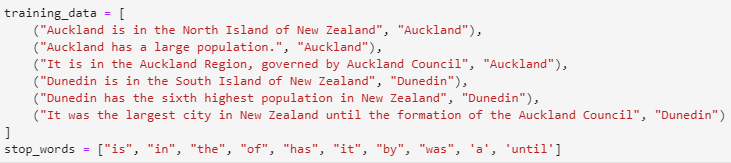
\includegraphics[width=0.8\textwidth]{../imgs/sentence_example.png}
        \caption{Six training observations in the format (sentence, label).}
    \end{figure}
\end{frame}

%-------------------------------------------------------------------------------
\begin{frame}{BoW Example}
 What does the training data look like after the stop words have been removed?
 \pause
    \begin{figure}
        \centering
        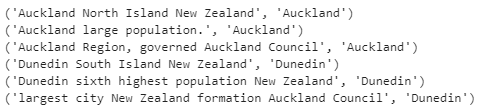
\includegraphics[width=0.8\textwidth]{../imgs/sentence_nostop.png}
        \caption{Training data with stop words removed.}
    \end{figure}
\end{frame}

%-------------------------------------------------------------------------------
\begin{frame}{BoW Example}
    What is the vocabulary in this example (the overall set of words)?\\
    \vspace{1em}
    
    $\{$ region, governed, highest, auckland, sixth, population, city, dunedin, formation, large, population, largest, south, council, island, north, zealand, new $\}$\\
    \vspace{1em}

    \textbf{New Zealand} and \textbf{new population} both add the counter for \textit{new} by 1, but do they mean the same?
\end{frame}

\begin{frame}{BoW Example}
    What are the priors for Auckland (A) and Dunedin (D)? ($p(A)$ and $p(D)$)
    \pause
    \begin{itemize}
        \item 6 training sentences.
        \item 3 labeled A, so $p(A) = \frac{3}{6} = 0.5$
        \item 3 labeled D, so $p(D) = \frac{3}{6} = 0.5$
    \end{itemize}
\end{frame}

%-------------------------------------------------------------------------------
\begin{frame}{BoW Example}
 What is the likelihood of seeing the word "Auckland" in a sentence labeled Auckland (A)? Dunedin (D)? ($p("Auckland"|A)$ and $p("Auckland"|D)$)
 \pause
 \begin{itemize}
     \item The training data has 13 words in total labeled with "A".
     \item 4 words labeled "A" are the word "Auckland".
     \item $p("Auckland"|A) = \frac{4}{13}$
     \pause
     \item The training data has 18 words in total labeled with "D".
     \item 1 word labeled "D" is the word "Auckland".
     \item $p("Auckland"|D) = \frac{1}{18}$
 \end{itemize}
\end{frame}

%-------------------------------------------------------------------------------    
\begin{frame}{BoW Problem}
 What is the likelihood of seeing the word "North" in a sentence labeled Auckland (A)? Dunedin (D)? ($p("North"|A)$ and $p("North"|D)$)
 \pause
 \begin{itemize}
     \item The training data has 13 words in total labeled with "A".
     \item 1 words labeled "A" are the word "North".
     \item $p("North"|A) = \frac{1}{13}$
     \item The training data has 18 words in total labeled with "D".
     \item 0 words labeled "D" are the word "North".
     \item $p("North"|D) = \frac{0}{18} = 0$
 \end{itemize}
 What happens when we try to calculate probabilities for a sentence with the word "North" in it?
\end{frame}

%-------------------------------------------------------------------------------
\begin{frame}{0 Probabilities}
    \begin{itemize}
        \item Since we multiply probabilities, and 0 encountered means the final probability will also be 0.
        \item The sentence "North Dunedin" would have get 0 probability for both Auckland and Dunedin!
        \item We can fix this with \textit{smoothing}, adding a small constant to the count of each word, label pair. This means we get no 0 likelihoods.
    \end{itemize}
\end{frame}

%-------------------------------------------------------------------------------
\begin{frame}{BoW Example}
 Using smoothing with constant 1, what is the likelihood of seeing the word "Auckland" in a sentence labeled Auckland (A)? Dunedin (D)? ($p("Auckland"|A)$ and $p("Auckland"|D)$)
 \pause
 \begin{itemize}
     \item The training data has 13 words in total labeled with "A".
     \item Smoothing adds 1 to the total count per word in the vocab, so adds 18. Our total count is 13 + 18 = 31.
     \item 4 words labeled "A" are the word "Auckland", + 1 from smoothing = 5.
     \item $p("Auckland"|A) = \frac{5}{31}$
     \pause
     \item The training data has 18 words in total labeled with "D". We add 18 from smoothing, so the total count = 36.
     \item 1 word labeled "D" is the word "Auckland", + 1 from smoothing = 2.
     \item $p("Auckland"|D) = \frac{2}{36}$
 \end{itemize}
\end{frame}

%-------------------------------------------------------------------------------
\begin{frame}{BoW Example}
 Using smoothing with constant 1, what is the likelihood of seeing the word "North" in a sentence labeled Auckland (A)? Dunedin (D)? ($p("North"|A)$ and $p("North"|D)$)
 \pause
 \begin{itemize}
     \item The training data has 13 words in total labeled with "A".
     \item Smoothing adds 1 to the total count per word in the vocab, so adds 18. Our total count is 13 + 18 = 31.
     \item 1 words labeled "A" are the word "North", + 1 from smoothing = 2.
     \item $p("North"|A) = \frac{2}{31}$
     \pause
     \item The training data has 18 words in total labeled with "D". We add 18 from smoothing, so the total count = 36.
     \item 0 words labeled "D" are the word "North", + 1 from smoothing = 1.
     \item $p("North"|D) = \frac{1}{36}$
 \end{itemize}
 Now we can still calculate probabilities, even with words not seen in the training data for a label.
\end{frame}

%-------------------------------------------------------------------------------
\begin{frame}{BoW Example}
    Using smoothing, what label would Naive Bayes predict for the sentence: "Auckland is in the north of the North Island"?
    \pause
    \begin{itemize}
        \item The BoW representation of the sentence is $\{$"Auckland": 1, "North": 2, "Island": 1$\}$
        \item For label $v$, the posterior probability is given by:
        \item $p("Auckland"|v)\times p("North"|v) \times p("North"|v) \times p("Island"|v) \times p(v)$
        \item = $p("Auckland"|v)^1\times p("North"|v)^2 \times p("Island"|v)^1 \times p(v)$
        \pause
        \item For $v=Auckland$: $\frac{5}{31}\frac{2}{31}^2\frac{2}{31}\times 0.5 = 0.00002$
        \item For $v=Dunedin$: $\frac{1}{36}\frac{1}{36}^2\frac{2}{36}\times 0.5 = 0.0000006$
        \item The maximum posterior probability is for "v=Auckland", so we label the observations as "Auckland".
    \end{itemize}
\end{frame}

%-------------------------------------------------------------------------------
\begin{frame}{Naive Bayes problem - Numeric Instability}
    A common problem encountered when implementing a Naive Bayes classifier is numeric instability.
    \begin{itemize}
        \item Computers store the likelihoods we calculate as floating point numbers, which may have small inaccuracies.
        \item Because we are multiplying many small floating point numbers together, we can encounter \textbf{underflow}.
        \item This is when the number we calculate is too small to be properly represented.
        \item Underflow can lead to our calculating returning a 0 probability, even though it should be a small number.
        \item This may be more of a problem as the input text gets longer, or the total number of words gets larger, as both push the posterior probability to smaller results which are more likely to underflow.
    \end{itemize}
\end{frame}

%-------------------------------------------------------------------------------
\begin{frame}{Underflow}
\begin{figure}
    \centering
    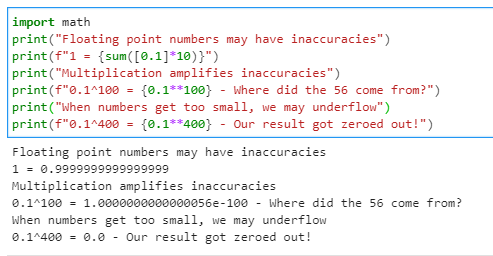
\includegraphics[width=0.8\textwidth]{../imgs/underflow.png}
    \caption{Example of underflow in python}
\end{figure}
\end{frame}
    
%-------------------------------------------------------------------------------
\begin{frame}{Log probabilities}
\begin{itemize}
    \item Underflow often occurs in Naive Bayes because we are multiplying many small numbers. How can we avoid it?
    \item We can covert our multiplication into an addition using log, as well as making our small probabilities larger numbers.
    \item $log(A\times B) = log(A) + log(B)$
    \item Logging an expression also maintains relative sizes. If $A > B$ then $log(A) > log(B)$.
    \item This means that if we take the log of our Naive Bayes expression, it won't change the relative posterior probabilities of the labels. I.E, we will still end up with the same selected label.
    \item $$\argmax_{v} p(v)\prod_{w_j}p(w_j|v) = \argmax_{v} log(p(v)) + \sum_{w_j}log(p(w_j|v))$$
\end{itemize}
\end{frame}

%-------------------------------------------------------------------------------
\begin{frame}{BoW Example}
    Using log probabilities, what label would Naive Bayes predict for the sentence: "Auckland is in the north of the North Island"?
    \pause
    \begin{itemize}
        \item The BoW representation of the sentence is $\{$"Auckland": 1, "North": 2, "Island": 1$\}$
        \item For label $v$, the posterior probability is given by:
        \item $log(p("Auckland"|v)) + log(p("North"|v)) + log(p("North"|v)) + log(p("Island"|v)) + log(p(v))$
        \pause
        \item For $v=Auckland$: $log(\frac{5}{31}) + 2log(\frac{2}{31}) + log(\frac{2}{31}) + log(0.5) = -4.66$
        \item For $v=Dunedin$: $log(\frac{1}{36}) + 2log(\frac{1}{36}) + log(\frac{2}{36}) + log(0.5) = -6.22$
        \item The maximum posterior probability is for "v=Auckland", so we label the observations as "Auckland".
    \end{itemize}
\end{frame}
    
%-------------------------------------------------------------------------------
\section{Extensions}
\begin{frame}{N-grams}
\begin{itemize}
    \item One problem we encounter with Naive Bayes is that we lose all interactions between features.
    \item Often interactions change the meaning of words, e.g., A news article with the words "machine" and "learning" could be to do with learning at school, so classified as 'education' whereas an article with the phrase "machine learning" is much more likely to be classified as 'tech'.
    \item We can introduce interactions by considering N-grams as features, instead of individual words.
    \item An N-gram is a sub-sequence of N words found in a text. Commonly we use bigrams (subsets of 2 words) and trigrams (subsets of 3 words).
\end{itemize}
\end{frame}

%-------------------------------------------------------------------------------
\begin{frame}{Bigram example}
\begin{itemize}
    \item What are the Bigrams of the sentence "Auckland is in the north of the North Island"? (including stop words)
    \pause
    \item \{"Auckland is", "is in", "in the", "the north", "north of", "of the", "the North", "North Island\}
    \item We have now captured the phrase "North Island" which is much more informative than "North" and "Island" separately!
\end{itemize}
\end{frame}

%-------------------------------------------------------------------------------
\begin{frame}{N-gram Problem}
\begin{itemize}
    \item What is a problem with N-grams?
    \pause
    \item We need \textit{more} training data to learn proper probabilities. We need to see multiple examples of all possible N length subsets for each label.
    \item It is much more likely to encounter an N-gram we haven't seen before than a single word!
\end{itemize}
\end{frame}

%-------------------------------------------------------------------------------
\begin{frame}{TF-IDF}
    \begin{itemize}
        \item Intuition - If a word appears in \textit{every} text, it is useless for telling the difference between classes.
        \item Alternatively, most highly informative words will not appear in very many texts. E.G, the word "rugby" may be relatively rare, but if we see it, it can tell us a lot about the sentence.
        \item We would like some way to place less weight on very common words, and more weight on rare words.
        \item This leads us to the idea of the ``document frequency" of a word. This is the proportion of documents (e.g, sentences in the training set) which contained a given word., with range [0, 1]. 0 Means the word appeared in no documents, 1 means it appeared in all documents.
        \item The log of the \textit{inverse} document frequency, can be thought of as the rarity of a word. $IDF_i = log(\frac{N}{D_i})$, where $N$ is the total number of documents and $D_i$ is the number of documents containing word $i$. We take the log so that IDF is 0 when the word appears in all documents, and grows slower as the word becomes rarer.
    \end{itemize}
\end{frame}

%-------------------------------------------------------------------------------
\begin{frame}{TF-IDF}
    \begin{itemize}
        \item In our BoW representation, we already calculate the frequency of each term.
        \item If we weight this count with the IDF for each word, we can take into account the rarity of each word.
    \end{itemize}
\end{frame}

%-------------------------------------------------------------------------------
\begin{frame}{TF-IDF example}
What are the IDF values associated with each word in the BoW example on slide 26?
\pause
    \begin{itemize}
        \item Auckland: $log(\frac{6}{4}) = 0.18$
        \item North: $log(\frac{6}{1}) = 0.78$
        \item Island: $log(\frac{6}{2}) = 0.48$
        \item New: $log(\frac{6}{4}) = 0.18$
        \item Zealand: $log(\frac{6}{4}) = 0.18$
        \item large: $log(\frac{6}{1}) = 0.78$
        \item population: $log(\frac{6}{2}) = 0.48$
        \item region: $log(\frac{6}{1}) = 0.78$
        \item governed: $log(\frac{6}{1}) = 0.78$
        \item council: $log(\frac{6}{2}) = 0.48$
        \item Dunedin: $log(\frac{6}{2}) = 0.48$
        \item south: $log(\frac{6}{1}) = 0.78$
        \item sixth: $log(\frac{6}{1}) = 0.78$
        \item highest: $log(\frac{6}{1}) = 0.78$
        \item \dots
    \end{itemize}
\end{frame}

%-------------------------------------------------------------------------------
\begin{frame}{TF-IDF example}
\begin{itemize}
    \item In order to use TF-IDF, we just replace any use of a words frequency with its frequency * IDF.
    \item Using smoothing we calculated $p(w_j|v) = \frac{f_{jv} + 1}{\sum_j(f_{jv}) +|V|}$, where $w_j$ is word $j$, $f_{jv}$ is the frequency of word $j$ in class $v$, and $|V|$ is the number of unique words in the vocabulary.
    \item Including TF-IDF, we calculate: $$
        p(w_j|v) = \frac{f_{jv}\times IDF_j + 1}{\sum_j(f_{jv}\times IDF_j) +|V|}
    $$
\end{itemize}
\end{frame}

\end{document}


